\documentclass[tikz,border=2mm]{standalone}
\usepackage{tikz}
\usetikzlibrary{arrows.meta,decorations.markings}

\begin{document}
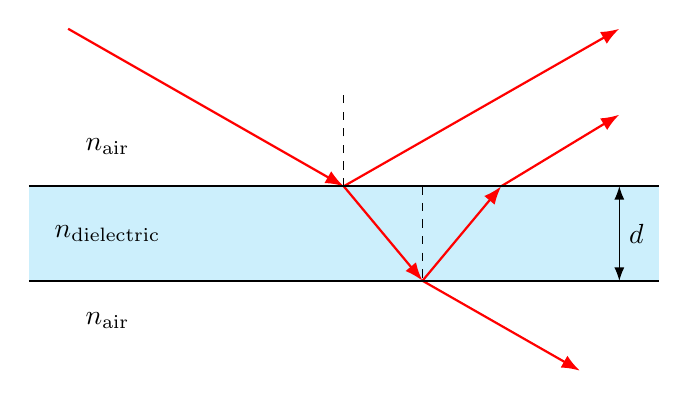
\begin{tikzpicture}[>=Latex, scale=1]


  \fill[cyan!20] (-4,0) rectangle (4,-1.2);

  \draw[dashed] (0,0) -- (0,1.2);
  \draw[dashed] (1,0) -- (1,-1.2);

  \draw[red, thick, ->] (-3.5,2) -- (0,0);
  \draw[red, thick, ->] (0,0) -- (3.5,2);
  \draw[red, thick, ->] (0,0) -- (1,-1.2);
  \draw[red, thick, ->] (1,-1.2) -- (3,-2.342857142857143);
  \draw[red, thick, ->] (1,-1.2) -- (2,0);

  \draw[red, thick, ->] (2,0) -- (3.5,0.9090909090);


  \node at (-3, 0.5) {$n_{\mathrm{air}}$};
  \node at (-3, -0.6) {$n_{\mathrm{dielectric}}$};
  \node at (-3, -1.7) {$n_{\mathrm{air}}$};


  \draw[<->] (3.5,0) -- node[right] {$d$} (3.5,-1.2);


    \draw[thick] (-4,0) -- (4,0);
    \draw[thick] (-4,-1.2) -- (4,-1.2);


\end{tikzpicture}
\end{document}